\definecolor{four1}{rgb}{0.21568627450980393,0.49411764705882355,0.7215686274509804}
\definecolor{four2}{rgb}{0.596078431372549,0.3058823529411765,0.6392156862745098}
\definecolor{four3}{rgb}{0.30196078431372547,0.6862745098039216,0.2901960784313726}
\definecolor{four4}{rgb}{0.8941176470588236,0.10196078431372549,0.10980392156862745}


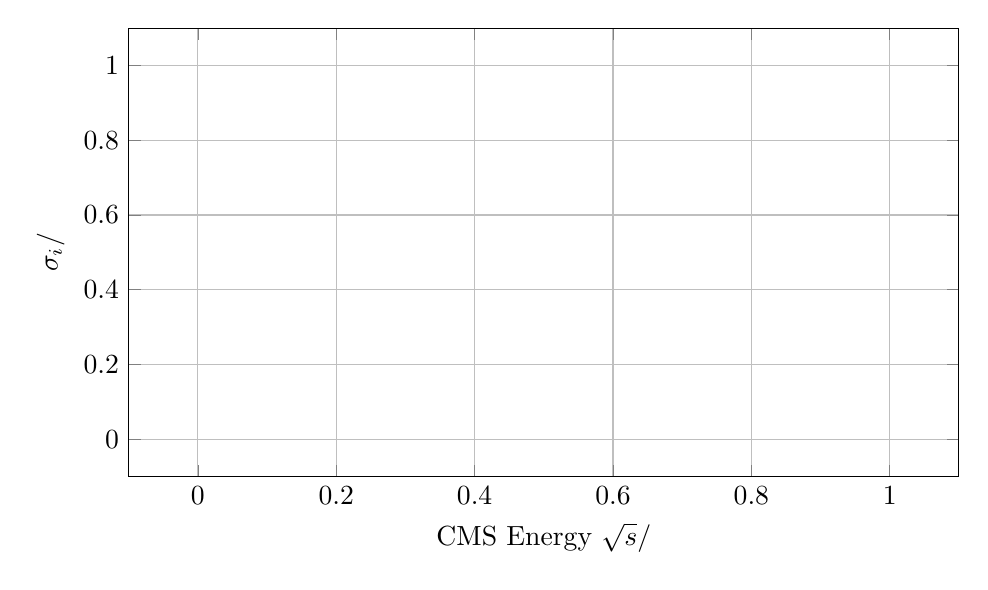
\begin{tikzpicture}
    \begin{axis}[
            width=\linewidth,
            height=0.6\linewidth,
            xlabel={CMS Energy $\sqrt{s} / \si{\giga\electronvolt}$},
            ylabel={$\sigma_i / \si{\nano\barn}$},
            grid=major,
            legend pos=north west,
        ]

%        \addplot[
%            electrons,
%            mark=*,
%            only marks,
%            error bars/y dir=both,
%            error bars/y explicit,
%        ] table[y error index=2] {../xy/cross_section-electrons.tsv};
%        \addlegendentry{Electrons}
%
%        \addplot[
%            muons,
%            mark=*,
%            only marks,
%            error bars/y dir=both,
%            error bars/y explicit,
%        ] table[y error index=2] {../xy/cross_section-muons.tsv};
%        \addlegendentry{Muons}
%
%        \addplot[
%            taus,
%            mark=*,
%            only marks,
%            error bars/y dir=both,
%            error bars/y explicit,
%        ] table[y error index=2] {../xy/cross_section-taus.tsv};
%        \addlegendentry{Taus}
%
%        \addplot[
%            hadrons,
%            mark=*,
%            only marks,
%            error bars/y dir=both,
%            error bars/y explicit,
%        ] table[y error index=2] {../xy/cross_section-hadrons.tsv};
%        \addlegendentry{Hadrons}
%
%        \addplot[electrons] table {../xy/cross_section-electrons-fit.tsv};
%        \addplot[muons] table {../xy/cross_section-muons-fit.tsv};
%        \addplot[taus] table {../xy/cross_section-taus-fit.tsv};
%        \addplot[hadrons] table {../xy/cross_section-hadrons-fit.tsv};

    \end{axis}
\end{tikzpicture}
